\chapter{CONCLUSIONS AND FUTURE WORK}
\thispagestyle{plain}

\label{Conclusions}

In the course of this dissertation, I have outlined the inner workings of the \framework.
The requirements and strategies for defining system-level properties were enumerated in Chapter \ref{Defining}.
The approach that \fw takes in solving the forward-mapping problem with regression was explained in Chapter \ref{ForwardMapping} and proven accurate and efficient in Chapter \ref{Results}.
Formulating the problem of prediction  system-level properties of an ABM as a regression problem leads to effecive prediction mechanisms.
The approach that \fw takes in solving the reverse-mapping problem with the novel simplical complex approach was explained in Chapter \ref{ReverseMapping} and proven accurate and efficient in most cases in Chapter \ref{Results}.
Inverting an approximation of the forward mapping proved to be an accurate and general way to build a reverse mapping to solve the reverse-mapping problem.

% The research project reached its aims
   % what did I try to achieve?
      % The main goal of the \framework is to bridge the gap between agent-level parameters and system-level properties.
The main goal of the \framework was to bridge the intuition gap between agent-level configuration parameters and system-level property values.
The forward mapping can be used by researchers to perform experimentation and is much faster than interacting with the ABM directly.
Whether the researcher is currently using an optimization approach or manually inspecting the system, using the forward mapping is  more convenient and faster than interacting with the ABM directly.
Only a small amount of error is incurred by using \fw, which is greatly outweighed by the benefits.
The reverse mapping can be used as a replacement for optimization and to provide the space of configurations that will satisfy a system-level property, which is useful for finding a number of configurations that will generate desired behavior in an ABM.
Also, researchers can use the reverse mapping as an aid to making qualitative conclusions about the nature of the system-level properties.

In Chapter \ref{Framework}, the following constraints were placed upon the implementation of \fw:
\begin{itemize}
      \item Domain-independent: The design of \fw should minimize the amount of configuration that is needed for each new domain;
      \item Algorithm-independent: any regression algorithm should be able to be applied with \fw;
      \item Accurate: \fw should generate accurate predictions and control suggestions; and
      \item Fast for the user: interactions with the models generated by \fw should require minimal computational time.
\end{itemize}

\fw achieved these goals. None of the four domains that \fw was applied required special modifications to the implementation of the framework in order to function correctly.
The same interfaces were used for each domain, and can be used for future domains.
The reverse-mapping solution simplical complex inversion is algorithm-independent, as shown by the fact that the core framework did not have to be modified in order to accommodate k-nearest neighbor, LOESS, or non-linear regression.
Future regression algorithms could be used for the forward mapping and the reverse mapping would require no changes.
Therefore, \fw is domain- and algorithm-independent.

The results in Chapter \ref{Results} show that the implementation of \fw produces accurate results across all of the domains that were tested.
In most cases, \fw was fast for the user.
From the results, forward mapping queries are thousands of times faster than actually querying the ABM.
This is important for researchers who wish to experiment with ABMs, but do not wish to spend upwards of eight seconds for each sample.
A query to the reverse mapping is typically lsss than two seconds; however, the response time does not scale well with dimensionality.
With higher dimensions, the reverse mapping is not fast for the user, and optimization or analyzing sub-portions of the configuration space should be considered as alternatives.
Therefore, \fw is accurate and efficient when dealing with low-dimensional behavior spaces.

In conclusion, the results show that \fw satisfies many of these constraints and satisfies the major goal of bridging the intuitive gap between agent-level configuration parameters and system-level property values.

\section{Future Work}

In the course of the research, a number of possible directions for future work have arisen.
Each of the following subsections discuss a possible subproblem in ABM meta-modeling or extensions to \fw that could produce interesting results.

\section{Extension: Specifying Ranges for System-level Properties}
\label{sec:ranges}

One of the major problems with SCI is that queries can easily become overspecified.
This is the case if the number of system-level properties exceeds the number of configuration parameters.
In the case of overspecification, the reverse mapping will not return any solutions, since they do not exist.
To avoid this problem, SCI could be altered to take as input \textit{ranges} of system-level property values, instead of specific values.
This would provide some leeway and allows for more possibility of intersections.
Instead of the solution of the reverse-mapping query being a hyperplane, it would become a hyperspace.
The query plane used to intersect with the reverse mapping would also be a hyperspace, bounded by two hyperplanes.

This extension would complicate the implementation significantly.
In order to implement this extension in SCI, the equations used would be inequalities, complicating the calculation of the intersection.
Any point that is satisfied by the set of inequalities over all simplexes could satisfy the system-level property ranges.
In the rest of this subsection, the QT approach is described, but the implementation is left as future work.

The Quad-Tree (QT) approach for inverting the forward mapping is intended to be simpler to implement than SCI.
Also, specifying ranges for system-level properties is more natural in QT than in SCI.
QT performs the same tasks as SCI, but instead returns a set of subspaces that must or could possibly contain configurations that satisfy the desired system-level property configuration.
In general, a quad-tree is a tree data structure in which each node either has zero or four children.
A quad-tree can be used to iteratively segregate a two-dimensional space into several subspaces in order to give certain portions of the space more detail.
Quad-trees use a notion of ``black," ``gray," and ``white" cells: black cells represent a subspace in which all values are black, white cells represent a subspace in which all values are white; and gray cells represent a subspace in which some values are white and some values are black.
The benefit of using a quad-tree structure is that black and white cells do not need to be expanded, as all of their values are already determined.
However, gray cells are broken down further by segregating its space into four children, which may be black, gray, or white.
Grey cells can be broken down as many times as desired, but typically, quad-trees are capped at a certain depth, which I call the ``granularity depth."

The idea of quad-trees can be used in the reverse mapping to approximate the solution space.
Black nodes are ones in which all values within the subspace match the query;
white nodes are ones in which none of the values within the subspace match the query;
and gray nodes are ones in which some of the values within the subspace match the query.
Instead of using squares to split the subspaces, QT must use hypercubes, since the configuration space is typically not two-dimensional.
QT returns all the gray cells and black cells found by this approach as an answer to a user's query.

Gray nodes are broken down iteratively until the granularity depth is reached.
QT breaks down a hypercube (a pair of simplexes) by querying the forward mapping for the points needed to break a single $n$-dimensional hypercube into $2^n$ hypercubes (split a line into two lines, a square into four squares, a cube into eight cubes, etc.).
Each new hypercube is then evaluated to see whether it contains the desired system-level property values or not, which can be determined by comparing the desired system-level property with the observed maximum and minimum among the corners of each hypercube.
If the desired system-level property value is less than the maximum, and greater than the minimum, then possibly an intersection satisfying all system-level properties exists within this hypercube.
If one of the values is not contained within this range, then the hypercube is marked as ``white" and does not need to be expanded further.

This approach has the benefit that the intersections of hyperplanes do not need to be calculated, which may be difficult to implement.
Although it is less accurate and the space it returns is not continuous, it serves the purpose of the reverse mapping in many ways.
It still returns configurations that the user should use to generate the behavior and can still be visualized to show the nature of the configurations that generate a particular system-level property.

Another motivation for using QT over SCI is that specifying ranges for system-level properties is difficult to represent in SCI because all of the equations are inequalities.
Meanwhile, the implementation in QT is quite simple because hypercubes either do or do not contain the target values.
Details on the uses of ranges in querying the reverse mapping are discussed in Section \ref{sec:ranges}.

\begin{figure}[ht]
\centering
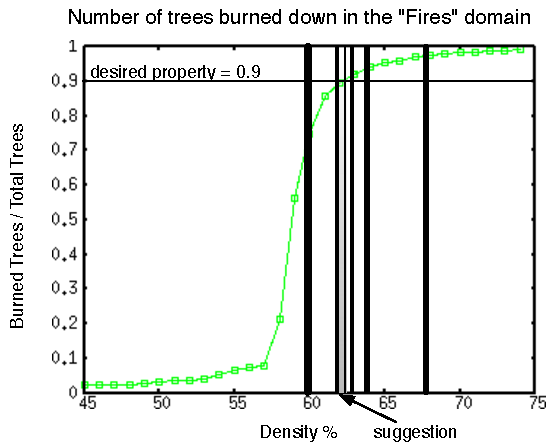
\includegraphics[scale=1]{images/QTfires.pdf}
\caption{The subspaces generated by QT represent a range of configurations that are close to satisfying the desired system-level property.}
\label{fig:qtfires}
\end{figure}

The usage of QT on the fires domain is visualized in Figure \ref{fig:qtfires}.
The thicker bars represent earlier subdivisions.
First, the space was split into the ranges 45--60 and 60--75.
The system-level property ranges from .02 to .7 in the 45--60 subspace, so this space can be ignored in future divisions because it does not contain the value .9.
The other half is subdivided at 67.5.
This process continues five times, which is the granularity depth in this case.
In a situation in which several solutions are possible, several subspaces will be returned as candidate configuration spaces.


\begin{figure}[ht]
\centering
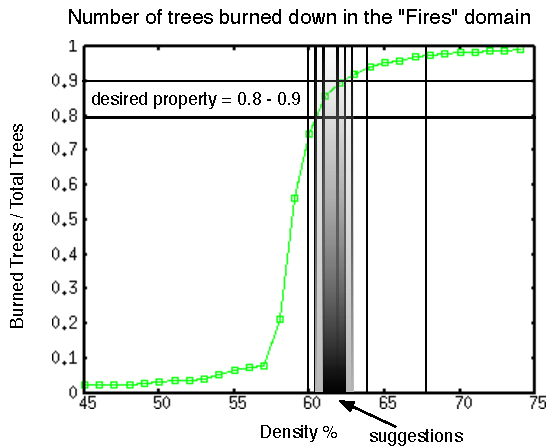
\includegraphics[scale=1]{images/QTfiresranges.pdf}
\caption{The subspaces generated by QT represent a range of configurations that are close to satisfying ranges of the desired system-level property.}
\label{fig:qtfiresranges}
\end{figure}
To handle ranges of system-level property values, only minor modifications to QT must be done.
The space is subdivided in the same way as standard QT; however, spaces that lie entirely within the ranged are marked as ``black" and do not need to be subdivided further.
Ranges marked as ``white" do not need to be subdivided either.
Gray areas are inspected more closely in order to increase the detail of the reverse mapping solution.
A set of configuration spaces is returned, representing the configurations that will satisfy the system-level property range.
This process is visualized in Figure \ref{fig:qtfiresranges}.



The caveat with this approach is that in non-monotonically changing domains, the maximum and minimum values at the corners do not necessary accurately describe the maximum and minimum within the hypercube.
If there exists a local minima or local maxima within a cube, the feature will be ignored.
To avoid this problem, the starting grid of hypercubes should be sufficiently detailed.



\subsection{Extension: Adaptive Meta-models}

In some agent-based models, a hidden property may change over the course of several runs, or perhaps within a same run, over time.
A hidden property is a feature of the environment that changes the behavior of the agents in some way, but is not directly detectable.
In the case that the hidden property does not change, the learned mappings will adapt to this hidden variable and the mappings will continue to be accurate.
However, in cases in which the hidden property changes over time, the learned mappings must be adaptive, since the value of the hidden property is not part of the configuration vector.
Because of a changing hidden property, the system-level behavior of a system can change, yet still be running the same configuration.

Wind in a flocking ABM serves as a good example of this phenomena.
A strong wind can change the behavior of a flocking system to be less cohesive.
However, the value of the wind is not predictable, which can cause predictions about the system to be erroneous.

To tackle this problem, the meta-models built by the forward and reverse mapping must be adaptive to the current conditions in the ABM.
I propose an online optimization technique that incrementally adjusts the behavior of the system to compensate for hidden changes in the system.
A continuous stream of current system-level property values will be provided as inputs into the framework.
The forward mapping will predict what should be happening with this configuration; this prediction would be compared to the actual system-level behavior.
The distance between the predicted and actual would be minimized by incrementally adjusting (i.e., hillclimbing or optimization) the configuration in order to minimize this gap.
Over time, the difference between the predicted and actual value will converge to zero.

The approach described here is an optimization approach, but is different from standard optimization because the initial starting position provided by the forward mapping is presumably close to the optimal configuration.
Also, the derivative of the mapping can be used in a gradient ascent approach, in which the derivative is calculated from the forward mapping.
Hidden variables typically will not change the nature of the system, only the specific values.
That is, increasing one configuration parameter is likely to have the same sort of effect regardless of hidden parameters, but not exactly.


% hidden properties that can change

\subsection{Correlated System-level Properties}
% need to predict all system-level properties as one.

One of the major assumptions used in the \fw approach to learning the reverse mapping is that the system-level property values are not correlated.
This assumption allows the reverse mapping problem to be split into a number of reverse mapping subproblems (one per system-level property).
However, if the properties are correlated, the result of the reverse mapping may be inaccurate.

For example, consider two system-level properties $a$ and $b$ are correlated such that $a \cdot b^2 = 1$.
Suppose that \fw, while solving the reverse-mapping problem, averages $a$ and $b$ separately for the following two instances: $a=100, b=\frac{1}{10}$ and $a=400, b=\frac{1}{20}$.
The averages are $a=250, b=\frac{1}{15}$; however, $250 \cdot \frac{1}{15} \neq 1$, which clearly is not a valid instance.

To avoid this problem, a multi-variate learning approach must be taken.
The forward mapping must be learned with a multi-variate regression algorithm, which must then be inverted in a multi-variate manner, as well.
This type of approach could consider all properties at once, and would therefore be immune to this problem.



\subsection{Handling Many Dimensions in Simplical Complex Inversion}

In Chapter \ref{Results}, the five-dimensional configuration space of the Wolf Sheep domain proved to be too large for simplical complex inversion.
I have considered a few approaches to tacking this problem in future work.

The first option is to use optimization instead of building a mapping.
This approach has the major problem that it will not return a space of solutions---it will only return one.
In many situations, this will be acceptable if the user is attempting to find a satisfactory configuration that will generate a specific system-level behavior.
An interesting point to note is that the behavior spaces are typically continuous.
Therefore, if there are many configurations that will satisfy the particular system-level property specification, they will probably exist near the point found with optimization.
A hillclimbing approach will move along these ridges of equal fitness and could return several possible configuration points.
This will work particularly well in situations in which the solution configuration space is linear, because the optimization simply follows a line.
However, with higher-dimensional configuration solution spaces, the representation of a hyperplanar solution space would be difficult to develop. 

Another approach to the problem would be to dynamically generate the majority of the simplical complex at run time.
This approach would allow a smaller portion of the mapping to reside in memory, making this problem far more tractable.
A specific simplex can contains a desired system-level property if the system-level property is within the minimum and maximum values of the simplex's corners.
These candidates can be broken up further to generate a more accurate mapping of the configuration solution space.
The major difficulty in this approach is the existence of local minima and local maxima within a simplex.
Consider the following example: a simplex has a minimum system-level property value of 4 and a maximum system-level property value of 6.
The value being sought is 7.
It is quite possible that at some point in the forward mapping, the value of the system-level property reaches 8, then decreases back down to 7 at the edge of the simplex.
It is impossible to determine that this is the case from just the values of the simplex corners.
One way in which a local maxima (or minima) could be inferred to exist within a simplex is to approximate the derivative (i.e., rate of change) of the system-level property at the edges of the simplex.
For example, if at all edges, the system-level property is increasing, then it is highly likely that a system-level property local maximum exists within this simplex.
The derivative can be approximated by viewing the values of other knots nearby, or by sampling additional points to approximate the derivative.
The domains I sampled and many of the domains discussed in Chapter \ref{RelatedWork} do not exhibit behavior spaces with many local minima and maxima.
Typically, the system-level property increases monotonically or has a single maximum, as the configuration changes.
Therefore, the simplex-based approach in approximating the derivative would likely be successful, since there are typically  only a limited number of maximums.

Although many approaches can be applied to reduce the computational complexity of solving the reverse problem, most approaches will suffer the curse of dimensionality, as does SCI.
As more dimensions are added, optimization techniques will have to search more of the space and SCI-type approaches will require more subspaces.
Even approaches similar to non-linear regression, which can be functionally inverted, become more complex with more dimensions.
With NLR, more model parameters and more variables make the system of equations significantly more difficult to solve.
Regardless of scaling issues, any improvement of performance in solving the reverse-mapping problem will allow researchers to inspect and analyze more complex agent-based models.

\subsection{Optimization of a System-Level Property}

In some cases, researchers may not want a configuration that produces a specific system-level behavior, but instead produces ``the best" system-level behavior.
In this case, an optimization approach, similar to that in work by Stonedahl and Wilensky (2010)\nocite{stonedahl}, could be used to find an optimal behavior.
A SCI-type approach would not be needed, because typically an ``optimal" behavior will be a single point, and does not necessarily need to be represented as a hyperplane.

Using the forward mapping could greatly improve the performance of work similar to that of Stonedahl and Wilensky, since instead of interacting with the ABM directly to calculate the fitness function, the optimization algorithm would be interacting with the forward mapping.
This method would greatly reduce the computation time of a particular optimization, at the cost of spending a significant amount of time training the forward mapping.
If many optimizations are to be performed, training the forward mapping would save time in the long run, since it can be used as many times as needed.
Instead, in a traditional optimization approach, the ABM would have to be re-sampled every time, even if the space being searched is the same as previous search spaces.


\section{Closing Thoughts}

It is my hope that this dissertation will spur additional research projects and discussions in tackling the problem of more efficient experimentation and deeper analysis of agent-based models.
This dissertation not only served to document for my particular approach and implementation, but also defined a number of core problems in this field.
Many alternative implementations are possible, some of which have been outlined in the Future Work section of this chapter.
Researching these additional solutions  will  lead to the discovery of new advances in the analysis of agent-based models.
Additional tools and theory regarding analysis of agent-based models will improve their usefulness in current models and their applicability to newer, more complex systems.


